% \documentclass[10pt, handout]{beamer}
\documentclass[10pt,aspectratio=169]{beamer}

\def\elementsroot{}\def\flatpack{}\usepackage{AOpres5h}
\usepackage{listings}\lstset{
    language=Java,
    basicstyle=\scriptsize,
    breaklines=true,
    tabsize=4,}
    
\title{\textsc{Flash-MAS} -- A Flexible and Lightweight Agent Shell}
% \author{}
\institute{}
\date{\today}

%------------------------------------------------
\setcontents{.1}
% \setlogos{\logoCS[.15\ph]}{\logoCStext}{\logoUPB[.07\ph]}{\logoAIMAS[.035\ph] \hskip.5cm \logoLIP[.06\ph]}

%-----------------------------

\begin{document}
\ignoreslidenumber\dotitlepage\ignoreslidenumber\docontentspage[.6\pw]\modeheadline


\section[Hello World]{Hello World -- A simple Java agent}

\subsection{Hello World Agent}
\begin{frame}[fragile]

\begin{itemize}
    \item An agent must extend the \code{flash.core.agent.Agent} interface, which extends the \code{Entity} interfce.
    \item To create an agent more easily one can extend the \code{flash.core.agent.BaseAgent} class and override the \code{start()} method.
\end{itemize}

    

\begin{lstlisting}
import net.xqhs.flash.core.agent.BaseAgent;

public class HelloWorldAgent extends BaseAgent {
	public boolean start() {
		if(!super.start()) return false;
		li("Hello World");
		stop();
		return true;
	}
}
\end{lstlisting}

{\small This code snippet is based on \code{example.helloWorld.HelloWorldAgent} in the \code{src-examples} source folder.}

\end{frame}

% new slide
\subsection{Starting the agent}
\begin{frame}[fragile]

Main startup options summary: 

\begin{itemize}
    \item via command line arguments: \\
        \code{java -cp "bin:lib-all/*" quick.Boot -agent HelloWorldAgent classpath:example.helloWorld.HelloWorldAgent}

    \item via XML deployment file: \\
        \code{java -cp "bin:lib-all/*" quick.Boot src-examples/example/helloWorld/deployment.xml}
\end{itemize}


    
\end{frame}

% subsections
% sending parameters
% receiving parameters

\section[Configuration]{Configuring entities}

\subsection{Sending parameters}
\begin{frame}[fragile]

% TODO titlu cu bold "Sending parameters via CLI" și pentru XML
% bullet și figură pe același slide
% folosește [fragile] doar când ai lstlisting în slide
% fără environment figure

% TODO la receiving: simplificat codul, la fel bullet + cod pe același slide



% The parameters of an entity can be \emph{sent} via the following two variants:

% \begin{itemize}
%     \item in a deployment configured via the command line. Figure~\ref{fig:configFigure} presents the configuration needed to start the deployment via command line arguments: the name of the agent, classpath and \code{stopAfter} parameters.
%     \item in a deployment configured in an XML deployment file. Figure~\ref{fig:func:deploymentXMLFile:code} presents the parameters needed to start a deployment via XML deployment file, being the same as above.
% \end{itemize}



\textbf{Sending parameters via CLI}

\begin{itemize}
    \item Configuration needed to start the deployment via command line arguments: the name of the agent, classpath and \code{stopAfter} parameters.
\end{itemize}


\centering
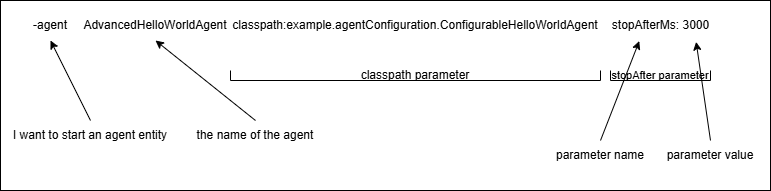
\includegraphics[width=\tw]{../img/config-figure.png}
  \label{fig:configFigure}

\end{frame}

\begin{frame}[fragile]

\textbf{Sending parameters via XML}

\begin{itemize}
    \item Configuration needed to start the deployment in an XML deployment file: the name of the agent, classpath and \code{stopAfter} parameters.
\end{itemize}

\begin{lstlisting}
<deployment>
    <agent classpath="example.agentConfiguration.ConfigurableHelloWorldAgent" name="HelloWorldAgent">
        <parameter name="stopAfterMs" value="3000"/>
    </agent>
</deployment>
\end{lstlisting}

{\small This code snippet is based on \code{example.agentConfiguration.deployment} in the \code{src-examples} source folder.}

\end{frame}



\subsection{Receiving parameters}
\begin{frame}[fragile]

\textbf{Receiving parameters by extending the \code{EntityCore} class}

\begin{itemize}
    \item The implementation uses the \code{getConfiguration()} method for extracting \code{stopAfter} parameter.
\end{itemize}

\begin{lstlisting}
public class ConfigurableHelloWorldAgent extends BaseAgent {

	public boolean start() {
		if(!super.start()) return false;
		
		long stopAfter = getConfiguration().get(STOP_AFTER_PARAMETER_NAME)).orElse(DEFAULT_STOP_AFTER);
		
		Timer t = new Timer();
		t.schedule(new TimerTask() {...}, stopAfter);
		return true;
	}
}
\end{lstlisting}

{\small This code snippet is based on \code{example.agentConfiguration.ConfigurableHelloWorldAgent} in the \code{src-examples} source folder.}


\end{frame}

\begin{frame}[fragile]

\textbf{Receiving parameters by overriding the \code{configure()} method}

\begin{itemize}
    \item The implementation overrides the \code{configure()} method and extracts the \code{stopAfter} parameter. The \code{configure()} method of an entity is called immediately after its construction.
\end{itemize}

\begin{lstlisting}
public class ConfigurableHelloWorldAgent2 extends BaseAgent {

	@Override
	public boolean configure(MultiTreeMap configuration) {
		if(configuration.isSet(STOP_AFTER_PARAMETER_NAME))
			stopAfter = configuration.getFirstValue(STOP_AFTER_PARAMETER_NAME);
		else
			stopAfter = DEFAULT_STOP_AFTER;
		return true;
	}
}
\end{lstlisting}

% {\small This code snippet is based on \code{package.package.package.ConfigurableHelloWorldAgent2} in the \code{src-examples} source folder.}

{\small This code snippet is based on \code{example.agentConfiguration.ConfigurableHelloWorldAgent2} in the \code{src-examples} source folder.}

\end{frame}


% \begin{frame}

% There are also two variants through which the parameters received in the configuration can be extracted by an entity:
% \begin{itemize}
%     \item extending the \code{EntityCore} class and using the \code{getConfiguration()} method. Figure~\ref{fig:func:ConfigurableHelloWorldAgent1:code} presents the code in this scenario. The implementation uses the \code{getConfiguration()} method for extracting \code{stopAfter} parameter.
%     \item overriding the \code{configure()} method. Figure~\ref{fig:func:ConfigurableHelloWorldAgent2:code} presents the code in this scenario. The implementation overrides the \code{configure()} method and extracts the \code{stopAfter} parameter. The \code{configure()} method of an entity is called immediately after its construction.
% \end{itemize}

% \end{frame}



\section[Messaging]{Messages between entities}

\subsection{Waves}
\begin{frame}

\begin{itemize}
    \item In \fmas[], an interaction between entities is performed via a \emph{wave}, implemented in the class \code{AgentWave}. 
    \item A wave has a \emph{source}, a \emph{destination}, and \emph{content}.
    \item  Waves are transmitted between entities either directly (via method calling) or by means of a communication infrastructure, which can transmit waves inside the same node or between different nodes.
    \item The source and destination are \emph{endpoints}.
    \item A \emph{message} is a wave sent between two agents, via a communication infrastructure.
    \item A \emph{Pylon} is an \emph{embodiment} of a communication infrastructure on a node.
    \item Interaction with a communication infrastructure is done directly (via proxy to the pylon) or via a \code{messagingShard}, which may be custom for the pylon implementation.
\end{itemize}

\end{frame}

\begin{frame}

\begin{itemize}
    \item UML class diagram of \code{AgentWave} in which the most important methods were included
\end{itemize}

\centering
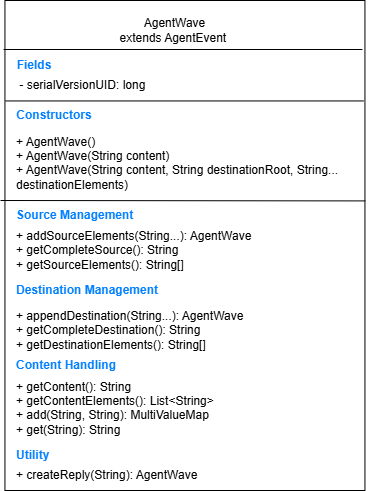
\includegraphics[scale=0.4]{../img/AgentWaveClassDiagram2.png}
  \label{fig:AgentWaveClassDiagram2}

\end{frame}



\subsection{Using communication pylons directly}

\begin{frame}

\textbf{Scenario for this example}

\begin{itemize}
    \item Two instances of the same agent class, \code{AgentPingPongPlain}, communicate back and forth by sending and receiving waves through a pylon, which is accessed by entities via a proxy (the \code{WaveMessagingPylonProxy} class).
    \item One instance is configured to act as the "ping" initiator (it has a \code{sendTo} parameter pointing to the other agent’s name), while the other implicitly becomes the "pong" responder (it has no \code{sendTo} parameter)
\end{itemize}

\end{frame}

\begin{frame}[fragile]

\textbf{Initialization}

\begin{itemize}
    \item The agent is placed, using information from the deployment configuration, in the context of the pylon. The pylon is visible by the agent via a proxy.
    \item When added in the context of the pylon, the agent \emph{registers} to the pylon, the communication infrastructure knows the node where the agent is located and the name of the agent, so it can receive messages.
    \item Agent must provide a proxy to the pylon, as a \code{WaveReceiver} instance.
\end{itemize}

\begin{lstlisting}
@Override
public boolean addContext(EntityProxy<Pylon> context) {
    pylonProxy = (WaveMessagingPylonProxy) context;
    return pylonProxy.register(getName(), new WaveReceiver() {
	   @Override
	   public void receive(AgentWave wave) {
		   processEvent(wave);
	   }
    })
}
\end{lstlisting}

{\small This code snippet is based on \code{testing.AgentPingPongPlain} in the \code{src} source folder.}


% cumva de marcat în același fel bulletul cu addConext / register / WaveReceiver și linia  / partea corespunzătoare din cod


% -- de arătat ce câmpuri / valori are wave-ul pe care l-ai construit în exemplu


\end{frame}


\begin{frame}[fragile]

\textbf{Sending messages}

\begin{itemize}
    \item The agent sends waves periodically using a timer.
    \item When the agent starts and it has a list of destinations, it schedules a task that sends a message to each destination every second.
\end{itemize}

\begin{lstlisting}
protected void sendPing() {
    AgentWave wave = new AgentWave("ping-no " + tick, otherAgent, "pong");
    pylonProxy.send(wave);
}
\end{lstlisting}

{\small This code snippet is based on \code{testing.AgentPingPongPlain} in the \code{src} source folder.}


\end{frame}

\begin{frame}[fragile]

\textbf{Receiving messages}

\begin{itemize}
    \item When an agent is registered to the pylon, it provides a receiver implementation that is triggered on incoming waves.
\end{itemize}

\begin{lstlisting}
protected boolean processEvent(AgentWave wave) {
    String replyContent = wave.getContent() + " reply";
    return send(wave.createReply(replyContent));
}
\end{lstlisting}

{\small This code snippet is based on \code{testing.AgentPingPongPlain} in the \code{src} source folder.}


\end{frame}

\subsection{Using communication pylons via messaging shards}

\begin{frame}[fragile]

\textbf{Scenario}

\begin{itemize}
    \item The agent delegates all messaging to a \code{MessagingShard} rather than using the \code{WaveMessagingPylonProxy} directly.
\end{itemize}

\textbf{Instantiating the Messaging shard} 

\begin{itemize}
    \item The shard is instantiated in the \code{register()} method using the \code{instantiateRecommendedShard()} method from the \code{AgentShardCore} class.
    \item After instantion, the shard is bound to the context, which gives it access to the messaging system through the proxy.
\end{itemize}

\begin{lstlisting}
msgShard = AgentShardCore.instantiateRecommendedShard(MESSAGING,
		(PylonProxy) context, null, new BaseAgentProxy() {
		   @Override
		   public boolean postAgentEvent(AgentEvent event) {
			   return processEvent(event)
		   }});
msgShard.addGeneralContext(context);
\end{lstlisting}

{\small This code snippet is based on \code{testing.AgentPingPong} in the \code{src} source folder.}


\end{frame}

\begin{frame}[fragile]

\textbf{Signaling start event} 

\begin{itemize}
    \item When the agent starts, it tells the shard by sending it an \code{AGENT\_START} event.
\end{itemize}

\begin{lstlisting}
@Override
public boolean start() {
    msgShard.signalAgentEvent(new AgentEvent(AgentEventType.AGENT_START));
}
\end{lstlisting}

{\small This code snippet is based on \code{testing.AgentPingPong} in the \code{src} source folder.}

\end{frame}


\begin{frame}[fragile]

\textbf{Sending messages} 

\begin{itemize}
    \item The \code{send()} method of the agent now simply delegates to the messaging shard.
    \item Internally, the shard adds the agent’s address to the wave if it is missing, and then forwards the message through either a \code{wavePylon} or a \code{classicPylon}, depending on what it has.
\end{itemize}

\begin{lstlisting}
msgShard.sendMessage(wave);
\end{lstlisting}

{\small This code snippet is based on \code{testing.AgentPingPong} in the \code{src} source folder.}

\end{frame}

\begin{frame}[fragile]

\textbf{Receiving messages} 

\begin{itemize}
    \item When a message arrives for the agent, the shard uses the proxy provided during registration.
    \item The proxy forwards the wave to the agent’s \code{processEvent()} method, presented in the first scenario.
\end{itemize}

\begin{lstlisting}
public boolean postAgentEvent(AgentEvent event) {
    return processEvent(event)
}
\end{lstlisting}

{\small This code snippet is based on \code{testing.AgentPingPong} in the \code{src} source folder.}


\end{frame}


\begin{frame}

\begin{itemize}
    \item Sequence diagram containing the agents, the pylon, and the shards
\end{itemize}

\centering
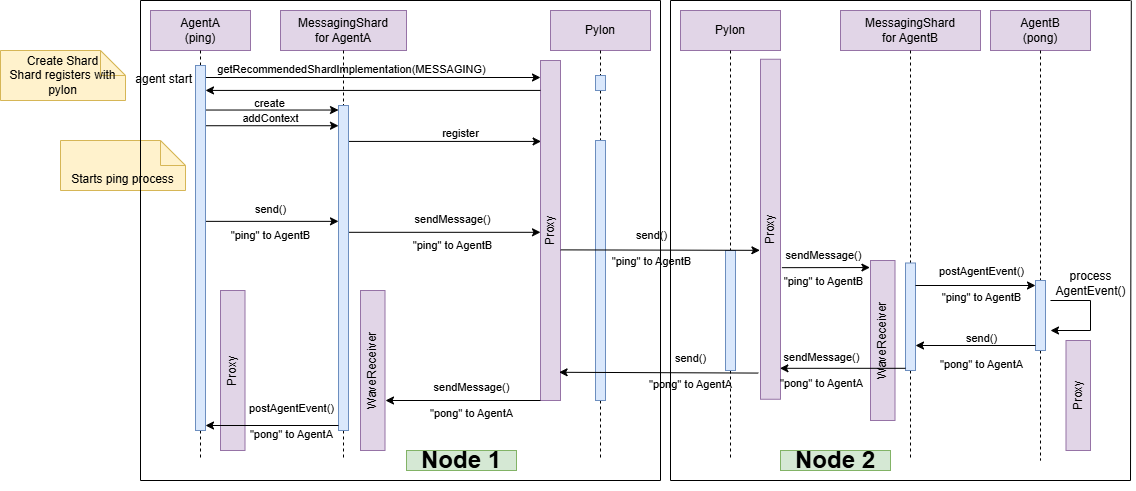
\includegraphics[width=\tw]{../img/AgentPingPongSequenceDiagramFinal.png}
  \label{fig:AgentPingPongSequenceDiagramFinal}

\end{frame}

\begin{frame}

\begin{itemize}
    \item UML class diagram for the agent - shard - pylon - pylon proxy - shard container structuring, especially from a context perspective
\end{itemize}

\centering
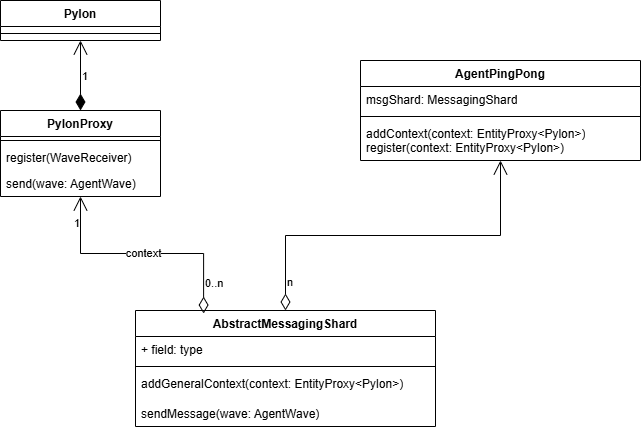
\includegraphics[scale=0.4]{../img/ContextStructureDiagram.png}
  \label{fig:ContextStructureDiagram}

\end{frame}



\subsection{Starting the deployment}
\begin{frame}

\begin{itemize}
    \item To start the deployment, one can run the \code{Boot} class from the \code{simplePingPong} subpackage under \code{src-examples/example}.
    \item In this file, one can select the desired interaction with the communication infrastructure, either directly using \code{AgentPingPongPlain}, or via a \code{messagingShard} by means of \code{AgentPingPong}. 
    \item Regardless of the option, the node, the names of the agents involved, the configuration of the \code{sendTo} parameter with the names of the agents that will receive messages, as well as the number of pings sent must be provided.
\end{itemize}

    
\end{frame}
 








\end{document}
